\chapter{Proposed system}

To be able to locate an object in 3D with no previous knowledge of the object (such
as its size, color and so on), two views of the same object are needed. The
views can be obtained by one moving camera or by multiple cameras. In this
thesis, we take a closer look at the second approach.

We propose a system with two cameras, connected via USB to a computer.
Two cameras provide enough information for object localization and make the
project usable also on low-budget. The placement of the cameras is important,
but no precise alignment is required. The cameras should share a significant part
of the view (see an example of the setup in the figure \ref{fig:camera-setup}).

\begin{figure}
	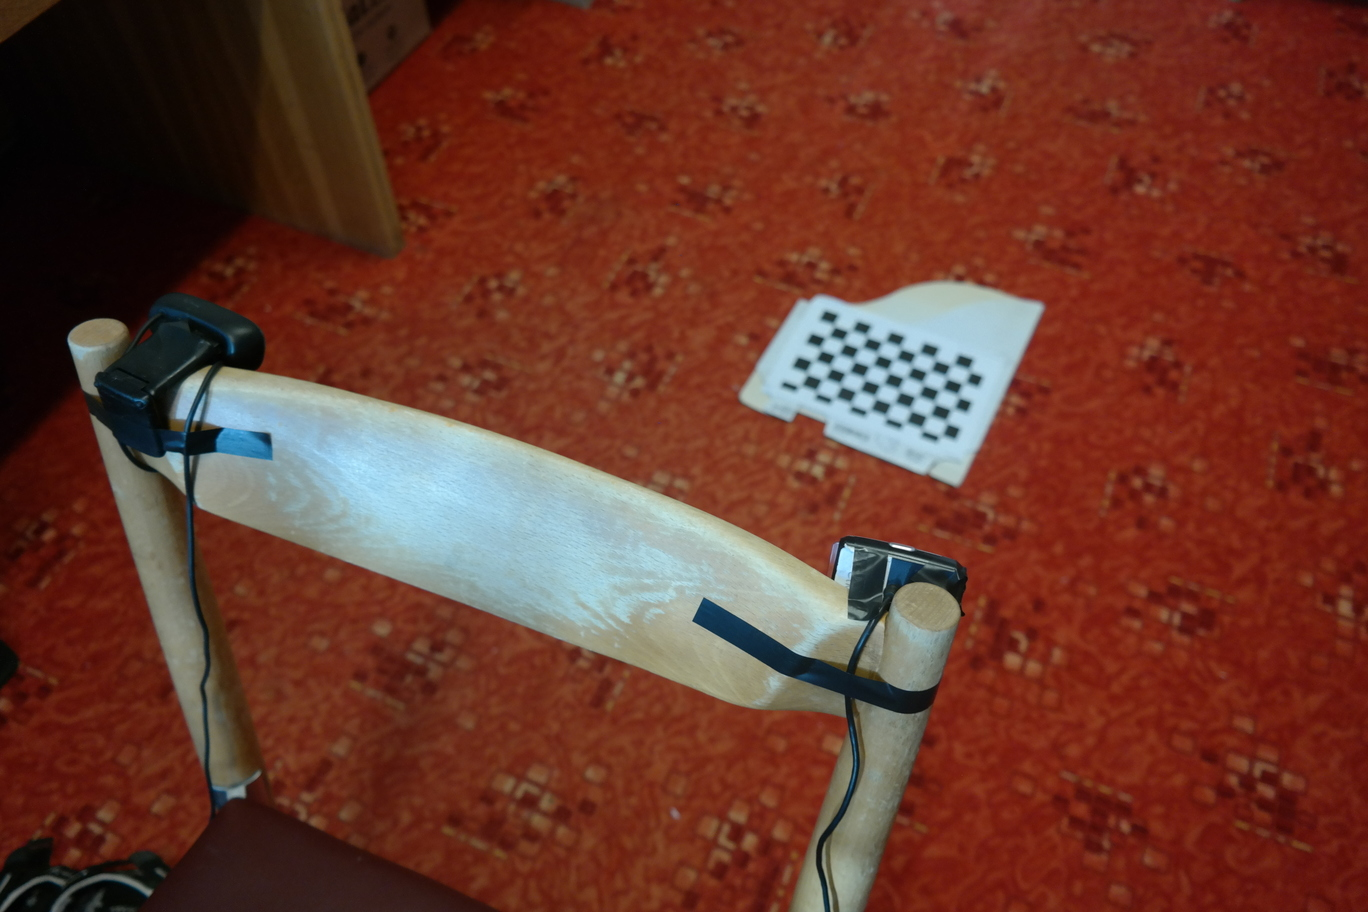
\includegraphics[width=\linewidth]{img/camera-positions.jpg}
	\caption{Example of camera setup}
	\label{fig:camera-setup}
\end{figure}

The program will be able to calibrate cameras to get their parameters. This
calibration will be based on showing a specific pattern to both cameras. From
this calibration, we obtain information for both cameras, but also their
distance to each other and the rotation between them.

After this calibration, the user marks the objects in both views of the
cameras. At this point, the tracker will start to estimate an object position
in camera view based on the images. We provide different tracker, so the user
can choose one to work with.

When we obtain information from calibration and the object position from both
images, we will estimate the object position in 3D space by simple linear
triangulation.

The each described step is crucial to get a system, which will be able to
localize point in 3D space. Each step is discussed separately in the following
chapter.

Now we provide a short insight into used tools and the notations, which are
used to describe our solution to the problem.

\section{Tools}

For the computer vision task, we use an \emph{OpenCV} library. OpenCV is an open
source computer vision library with many algorithms implemented (for example
calibration, triangulation, and so on). We use trackers which are now available
only in the \emph{contribute} version. For more information and examples of usage
visit their webpage\footnote{\url{https://opencv.org/}}.

To provide a comparison of trackers, we also include one tracker from
\emph{Dlib}\footnote{\url{http://dlib.net/}} library. It is also open source
and an interface for the Python is provided.  Since this library focus is on
machine learning, it does not contain as many functions for computer vision
as the OpenCV library yet.

\section{Notations}

The following section describes some procedures using math notion. To avoid
ambiguity we provide the overview of the used notation here.

\subsubsection*{Vector}
A word \emph{vector} denotes a column vector in a shape of $n\times1$.

\subsubsection*{Block matrix}
A matrix operation $W = (A|B)$, where $A$ is a matrix $m \times n$ and B is a
matrix $m \times p$, creates matrix $W$, where the first $n$ columns are the entries from
matrix $A$ and the last $p$ columns consist of the columns of matrix $B$.
Example:

\[
A = \begin{pmatrix}
        1 & 2 \\
        3 & 4
\end{pmatrix},
B = \begin{pmatrix}
5 \\
6
\end{pmatrix},
(A|B) = \begin{pmatrix}
        1 & 2 & 5 \\
        3 & 4 & 6
\end{pmatrix}
\]

\subsubsection*{Homogenous coordinates}

In computer vision, homogenous coordinates are used frequently instead of
Cartesian coordinates. Cartesian coordinates are the most common coordinate
system.  Homogenous coordinates have one element added. This element is a
scaling factor. As an example, vector $(2x, 2y, 2z, 2)^T$ represents same point
as $(x, y, z, 1)^T$ in homogenous coordinates. The same point is equal to $(x,
y, z)^T$ in Cartesian coordinates. Unlike the Cartesian coordinates, a single
point can be represented by infinitely many homogenous coordinates.

Similarly it works for coordinates in any n-dimensional space. In conversion
from Cartesian to homogenous coordinates we simply add a new element at the end
equal to one. In the opposite direction, we divide first $n-1$ values by the
$n$th.

In homogenous coordinates the origin is ommited. Homogenous coordinates provide
us also a way how to represent a point in the infinity by finite coordinates.
These points in the infinity are represented with the scale factor equal to 0.

This coordinates representation is tightly bounded to a projective plane, on
which the mathematical theory behind is based. For us, it is just important to
know how to convert them to Cartesian coodinates and that algorithms for
computer vision often use them.
